\documentclass[border=10pt]{standalone}
\usepackage{pgfplots}
\pgfplotsset{compat=1.18}
\begin{document}
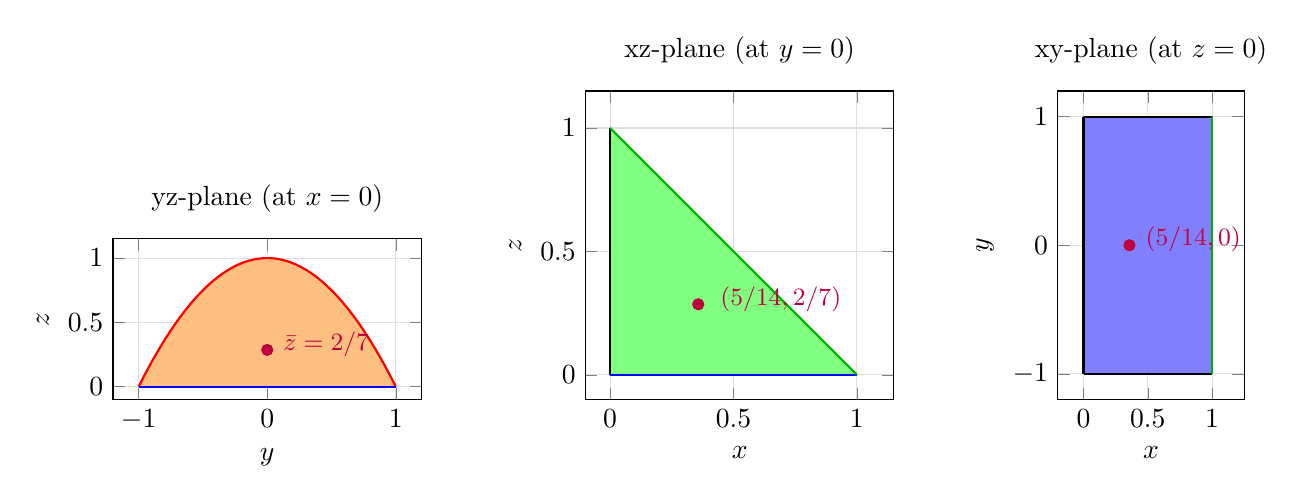
\begin{tikzpicture}
\begin{axis}[
    name=plot1,
    width=5.5cm, height=5.5cm,
    xlabel={$y$}, ylabel={$z$},
    title={yz-plane (at $x=0$)},
    xmin=-1.2, xmax=1.2, ymin=-0.1, ymax=1.15,
    axis equal image,
    grid=major, grid style={gray!25},
    at={(0,0)}
]
\addplot[orange!60, fill=orange!50, samples=50, domain=-1:1] (x, {1-x*x}) \closedcycle;
\addplot[red, thick, samples=50, domain=-1:1] (x, {1-x*x});
\addplot[blue, thick] coordinates {(-1, 0) (1, 0)};
\addplot[only marks, mark=*, mark size=2pt, color=purple] coordinates {(0, 2/7)};
\node[purple, anchor=west] at (axis cs:0.05, 2/7+0.04) {\small $\bar z = 2/7$};
\end{axis}
\begin{axis}[
    name=plot2,
    width=5.5cm, height=5.5cm,
    xlabel={$x$}, ylabel={$z$},
    title={xz-plane (at $y=0$)},
    xmin=-0.1, xmax=1.15, ymin=-0.1, ymax=1.15,
    axis equal image,
    grid=major, grid style={gray!25},
    at={(6cm,0)}
]
\addplot[green!60, fill=green!50] coordinates {(0,0) (1,0) (0,1)} \closedcycle;
\addplot[black, thick] coordinates {(0,0) (0,1)};
\addplot[blue, thick] coordinates {(0,0) (1,0)};
\addplot[green!70!black, thick] coordinates {(0,1) (1,0)};
\addplot[only marks, mark=*, mark size=2pt, color=purple] coordinates {(5/14, 2/7)};
\node[purple, anchor=west] at (axis cs:5/14+0.05, 2/7+0.02) {\small $(5/14, 2/7)$};
\end{axis}
\begin{axis}[
    name=plot3,
    width=5.5cm, height=5.5cm,
    xlabel={$x$}, ylabel={$y$},
    title={xy-plane (at $z=0$)},
    xmin=-0.2, xmax=1.25, ymin=-1.2, ymax=1.2,
    axis equal image,
    grid=major, grid style={gray!25},
    at={(12cm,0)}
]
\addplot[blue!60, fill=blue!50] coordinates {(0,-1) (1,-1) (1,1) (0,1)} \closedcycle;
\addplot[black, thick] coordinates {(0,-1) (1,-1)};
\addplot[black, thick] coordinates {(0,1) (1,1)};
\addplot[black, thick] coordinates {(0,-1) (0,1)};
\addplot[green!70!black, thick] coordinates {(1,-1) (1,1)};
\addplot[only marks, mark=*, mark size=2pt, color=purple] coordinates {(5/14, 0)};
\node[purple, anchor=west] at (axis cs:5/14+0.05, 0.05) {\small $(5/14, 0)$};
\end{axis}
\end{tikzpicture}
\end{document}